% --------------------------------------------------------------
% This is all preamble stuff that you don't have to worry about.
% Head down to where it says "Start here"
% --------------------------------------------------------------
 
\documentclass[12pt]{article}
 
\usepackage[margin=1in]{geometry} 
\usepackage{amsmath,amsthm,amssymb}
\usepackage{graphicx}
\usepackage{enumerate}
\usepackage{xcolor}
\definecolor{smithblue}{HTML}{002855}
\definecolor{smithyellow}{HTML}{F2A900}

\usepackage[parfill]{parskip}
\parskip=\baselineskip
 
\newcommand{\N}{\mathbb{N}}
\newcommand{\Z}{\mathbb{Z}}
 
\newenvironment{exercise}[2][Exercise]{\begin{trivlist}
\item[\hskip \labelsep {\bfseries #1}\hskip \labelsep {\bfseries #2.}]}{\end{trivlist}}

\newenvironment{solution}[1][{\color{red} Solution:}]{\begin{trivlist}
\item[\hskip \labelsep {\bfseries #1}\hskip \labelsep {\bfseries}]}{\end{trivlist}}

\usepackage{fancyhdr}
\pagestyle{fancy}
\lhead{Submitted by: \studentName\\
\collaborators}
\rhead{CSC250 Spring 2024 - Assignment 5\\
\today{}}
\cfoot{p. \thepage}
\renewcommand{\headrulewidth}{0.4pt}
\renewcommand{\footrulewidth}{0.4pt}
 
\begin{document}
 
% --------------------------------------------------------------
%                         Start here
% --------------------------------------------------------------

\newcommand{\studentName}{YOUR NAME HERE} %replace with your name

\newcommand{\collaborators}{
	% Comment out the line below if you worked alone
	with \textit{COLLABORATORS' NAMES HERE}
	% Uncomment the line below if you worked alone
	% \textit{I did not collaborate with anyone on this assignment.}
}

% --------------
% Exercise 1
% --------------
\begin{exercise}{1}

Answer each of the following questions, and explain your reasoning.
\begin{enumerate}[(a)]
	\setlength{\itemsep}{10em}
	\item Can a Turing Machine ever write the blank symbol $\square$ on its tape?
	% -------------------------------------------
	%  Write your answer to Q1a below
	% -------------------------------------------
	\begin{solution}
	\end{solution}
	
	\item Can the tape alphabet $\Gamma$ be the same as the input alphabet?
	% -------------------------------------------
	%  Write your answer to Q1b below
	% -------------------------------------------
	\begin{solution}
	\end{solution}
	
	\item Can a Turing Machine's head ever stay in the same location for two steps back to back?
	% -------------------------------------------
	%  Write your answer to Q1c below
	% -------------------------------------------
	\begin{solution}
	\end{solution}
	
	\item Can a Turing Machine contain just a single state?
	% -------------------------------------------
	%  Write your answer to Q1d below
	% -------------------------------------------
	\begin{solution}
	\end{solution}
\end{enumerate}
\end{exercise}

\clearpage

% \vskip 2em 
% \hrule
% \vskip 2em 

% --------------
% Exercise 4
% --------------
\begin{exercise}{2}
Show that the set of \textbf{decidable} languages is closed under:
\begin{enumerate}[(a)]
	\setlength{\itemsep}{15em}
	\item union
	% -------------------------------------------
	%  Write your answer to Q2a below
	% -------------------------------------------
	\begin{solution}
	\end{solution}
	
	\item intersection
	% -------------------------------------------
	%  Write your answer to Q2b below
	% -------------------------------------------
	\begin{solution}
	\end{solution}
	
	\item complement
	% -------------------------------------------
	%  Write your answer to Q2c below
	% -------------------------------------------
	\begin{solution}
	\end{solution}
\end{enumerate}
\end{exercise}
\clearpage

% --------------
% Exercise 5
% --------------
\begin{exercise}{3}
Consider the following TM $M$ that decides the language $L = \{0^{2^n} | n \ge 0\}$
\footnotesize{\begin{verbatim}
M = "On input string w:
    1. Sweep left to right across the tape, crossing off every other 0.
    2. If in stage 1 the tape contained a single 0, ACCEPT.
    3. If in stage 1 the tape contained more than a single 0 
       and the number of 0s was odd, REJECT.
    4. Return the head to the left-land end of the tape.
    5. Go to stage 1."
\end{verbatim}}
We can describe this machine formally as:
\begin{eqnarray*}
Q &=& \{q_1, q_2, q_3, q_4, q_5, q_{accept}, q_{reject}\}\\
\Sigma &=& \{0\}\\
\Gamma &=& \{0,x,\square\}
\end{eqnarray*}
with start state $q_1$, accepting state $q_{accept}$ and rejecting state $q_{reject}$. We describe $\delta$ with the following diagram (Sipser, p. 144):
\begin{center}
\vspace{-1em}
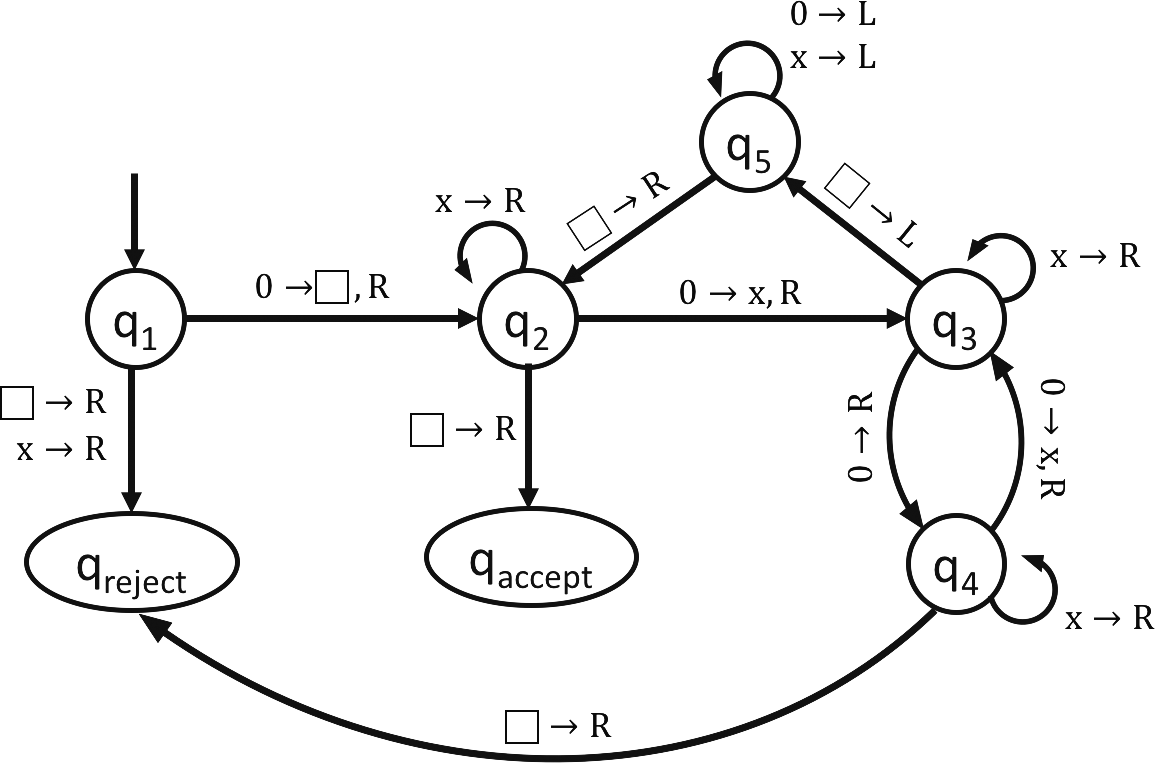
\includegraphics[width=0.6\textwidth]{e2.png}
\end{center}
Give the sequence of configurations that $M$ enters when started on each of the following strings:
\begin{enumerate}[(a)]
	\setlength{\itemsep}{15em}
	\item 0
	\vfill\hfill\textit{...continued on next page.}
	% -------------------------------------------
	%  Write your answer to Q3a below
	% -------------------------------------------
	\begin{solution}
	\end{solution}
	
	\item 00
	% -------------------------------------------
	%  Write your answer to Q3b below
	% -------------------------------------------
	\begin{solution}
	\end{solution}
	
	\item 000
	% -------------------------------------------
	%  Write your answer to Q3c below
	% -------------------------------------------
	\begin{solution}
	\end{solution}
	
	\item 000000
	% -------------------------------------------
	%  Write your answer to Q3d below
	% -------------------------------------------
	\begin{solution}
	\end{solution}
	
\end{enumerate}
\end{exercise}
\clearpage

% --------------
% Exercise 4
% --------------
\begin{exercise}{4}
Show that the following language is \textbf{decidable}:
\[\{\langle A \rangle \ | \ A \texttt{ is a DFA and } L(A) \texttt{ is infinite}\}\]
\textit{Hint: consider what you know about DFAs and their languages...}
% -------------------------------------------
%  Write your answer to Q4 below
% -------------------------------------------
\begin{solution}
\end{solution}

\end{exercise}

\clearpage
% \vskip 2em 
% \hrule
% \vskip 2em 

% --------------
% Exercise 5
% --------------
\begin{exercise}{5 \textbf{OPTIONAL}}
A Turing machine with STAY PUT instead of LEFT  is similar to an ordinary Turing machine, but the transition function has the form:
\[\delta:Q\times\Gamma \rightarrow Q \times \Gamma \times \{R,S\}\]
At each point the machine can move its head right or let it stay in the same position on the tape. Show that this Turing machine variant is \textbf{not equivalent} to the usual version. What class of languages do these machines recognize?
\end{exercise}

% -------------------------------------------
%  Write your answer to Q5 below
% -------------------------------------------
\begin{solution}
\end{solution}

% -----------------
% References
% -----------------
\vfill
\begin{thebibliography}{9}
 
\end{thebibliography}

% --------------------------------------------------------------
%     You don't have to mess with anything below this line.
% --------------------------------------------------------------
 
\end{document}